% Chapter Template

\chapter{Methodology} % Main chapter title

\label{Chapter 3} % Change X to a consecutive number; for referencing this chapter elsewhere, use \ref{ChapterX}

\lhead{Chapter 3. \emph{Methodology}} % Change X to a consecutive number; this is for the header on each page - perhaps a shortened title

\section{Overview}

This project employs an extended multi-agent clinical simulation framework designed to evaluate large language models (LLMs) under interactive, multi-turn diagnostic conditions. Unlike static question–answer paradigms, the system models realistic doctor–patient encounters through structured dialogue, selective evidence acquisition, and controlled behavioural variations. The framework integrates four specialized agents—Doctor, Patient, Measurement, and Evaluator—coordinated by a deterministic interaction controller. Each agent is implemented as a role-conditioned LLM with its own instructions, behavioural constraints, and memory mechanisms. This modular design enables reproducible experimentation, robust evaluation, and fine-grained analysis of reasoning trajectories and bias effects.

\section{Scenario Loading and Case Construction}

Evaluation begins with the loading of structured medical scenarios from curated datasets such as MedQA and extended clinical case repositories. Scenario loaders (e.g., \texttt{ScenarioLoaderMedQA}) parse each case into its fundamental components:
\begin{itemize}
    \item patient background and demographic details,
    \item presenting complaints and symptom narratives,
    \item physical examination findings,
    \item diagnostic test results,
    \item ground-truth diagnosis.
\end{itemize}

Each scenario functions as a complete clinical vignette, ensuring consistency and comparability across model evaluations. These structured case representations serve as the foundation for each simulated interaction episode.

\section{Multi-Agent Simulation Loop}

A multi-turn simulation loop is executed for each scenario, consisting of repeated interactions among the Doctor, Patient, and Measurement Agents. The loop runs for a predefined number of iterations (typically ten) or until the doctor explicitly declares a diagnosis.

Figure~\ref{fig:agent-flowchart} illustrates the overall structure and information flow of the proposed multi-agent clinical simulation framework. The diagram highlights how each agent interacts with the others through the Interaction Orchestrator, and how diagnostic reasoning emerges through sequential doctor–patient dialogue, structured test retrieval, and final moderator-based evaluation.

\begin{figure}[H]
    \centering
    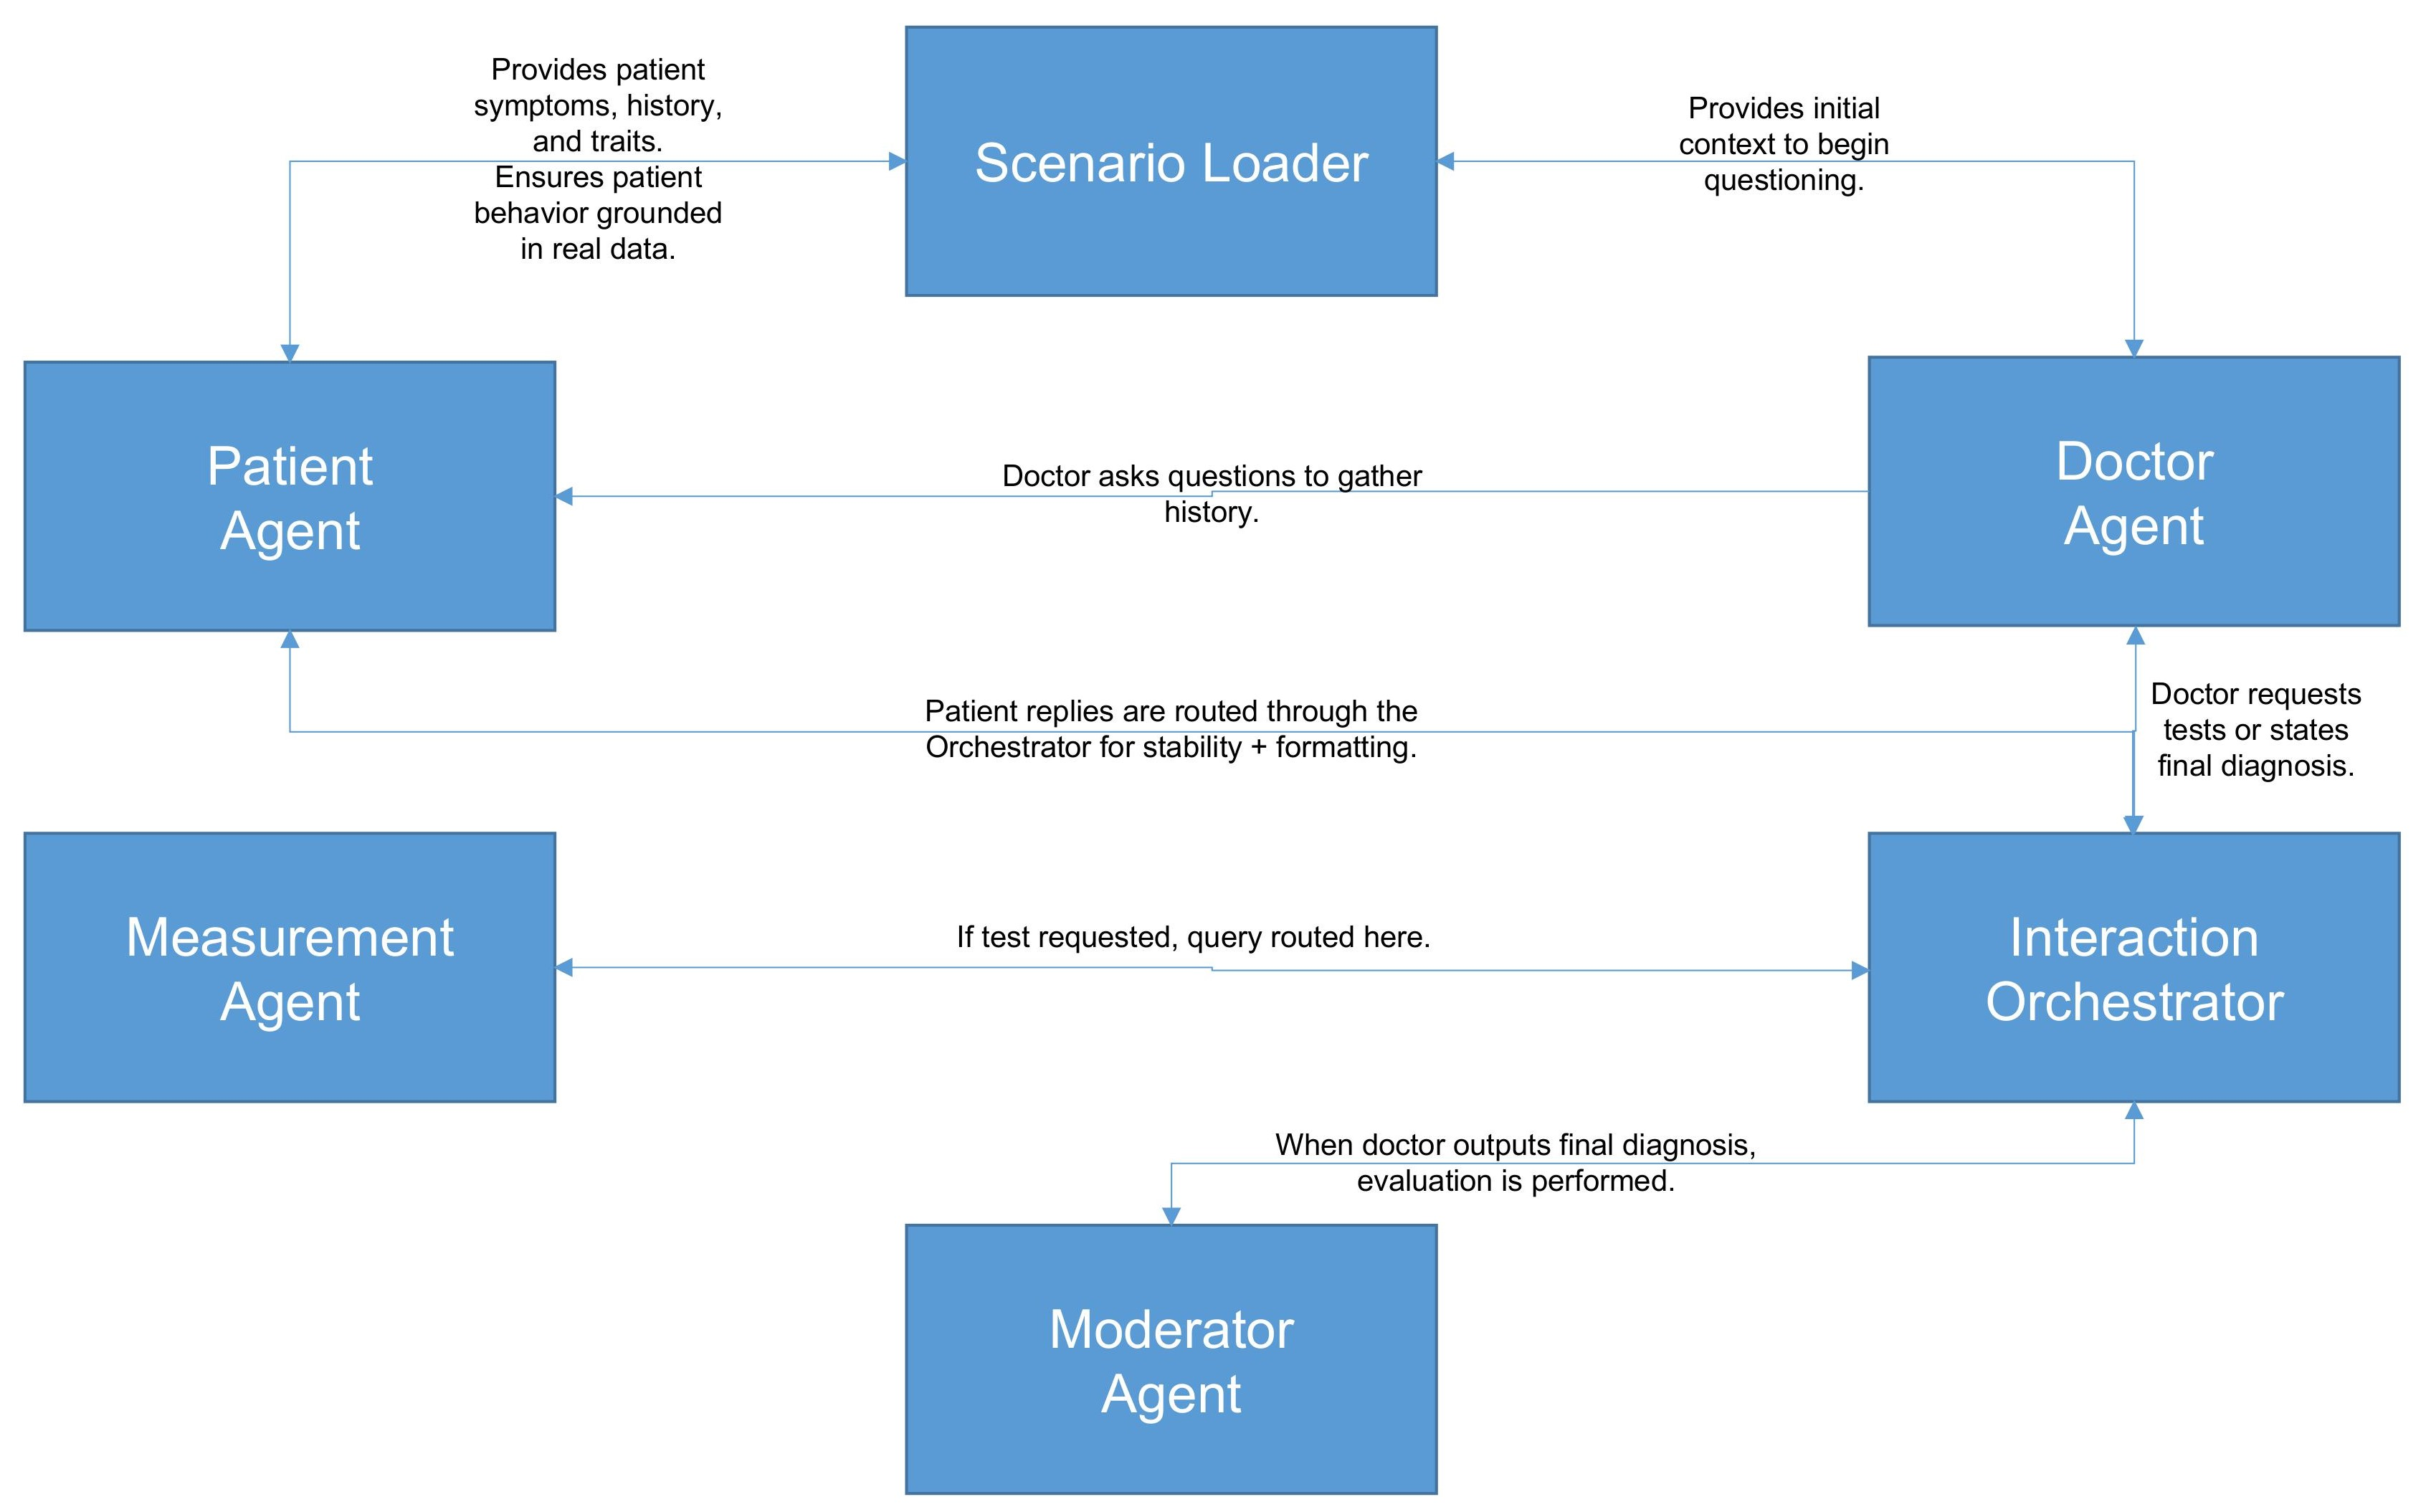
\includegraphics[width=\textwidth]{Pictures/Flowchart_pic.jpg}
    \caption{Overview of the multi-agent interaction workflow used in the proposed clinical simulation framework. 
    The Scenario Loader initializes each case and distributes case-specific information to the appropriate agents. 
    The Doctor Agent performs history-taking, hypothesis generation, and test ordering. 
    The Patient Agent produces symptom-grounded responses, while the Measurement Agent returns structured diagnostic tests upon request. 
    All communication flows through the Interaction Orchestrator, which ensures turn-taking, stability, and state management. 
    Once the Doctor provides a final diagnosis, the Moderator Agent evaluates its correctness through semantic comparison.}
    \label{fig:agent-flowchart}
\end{figure}



\subsection{Doctor Agent}

The Doctor Agent is the primary LLM being evaluated. It engages in:
\begin{itemize}
    \item history-taking and follow-up questioning,
    \item hypothesis formation and refinement,
    \item ordering of diagnostic tests,
    \item synthesis of a final diagnosis.
\end{itemize}

Its prompt is organized hierarchically to improve stability and ensure role fidelity. The doctor must communicate its final decision using the structured format:
\[
\texttt{DIAGNOSIS READY: <diagnosis>}
\]
This explicit signalling ensures deterministic extraction and evaluation of diagnostic predictions.

\subsection{Patient Agent}

The Patient Agent generates clinically grounded responses based on the scenario’s symptom structure. It provides concise (1–3 sentence) answers and may exhibit behavioural variations such as anxiety, guardedness, or verbosity, depending on configured bias conditions. The Patient Agent does not generate novel medical data; it remains anchored to the case specifications.

\subsection{Measurement Agent}

The Measurement Agent supplies structured diagnostic information only when the doctor explicitly requests a valid test. Supported modalities include:
\begin{itemize}
    \item vital signs,
    \item laboratory test panels,
    \item imaging study summaries,
    \item physical examination findings.
\end{itemize}

This agent prevents hallucinated or unsupported diagnostics by returning only scenario-derived information.

\subsection{Dialogue Orchestration}

A deterministic Interaction Orchestrator governs message routing, agent transitions, turn ordering, and termination conditions. Functionally, it operates as a finite-state controller with states representing history-taking, evidence acquisition, hypothesis refinement, and conclusion stages. It also handles output irregularities and ensures simulation integrity even when LLM outputs diverge or drift.

\section{Bias Injection Mechanism}

A distinctive component of the framework is its configurable bias-injection system, which enables controlled manipulation of behavioural tendencies in both the Doctor and Patient Agents.

\subsection{Patient-Side Bias}

Patient-side bias affects the tone, completeness, and clarity of responses. Configurable attributes include:
\begin{itemize}
    \item mistrust or guardedness,
    \item excessive confidence (self-diagnosis),
    \item emotional variability,
    \item demographic or cultural features.
\end{itemize}

These modifiers alter how the patient reports symptoms, potentially influencing the doctor's reasoning trajectory.

\subsection{Doctor-Side Cognitive Bias}

Doctor-side biases modify the internal reasoning patterns of the doctor. Examples include:
\begin{itemize}
    \item anchoring on early cues,
    \item confirmation-seeking behaviour,
    \item recency-weighted decision-making,
    \item premature diagnostic closure,
    \item overconfidence.
\end{itemize}

These cognitive distortions help evaluate whether the LLM remains robust under fallible reasoning conditions that mimic human diagnostic errors.

\section{Moderator-Based Evaluation}

Upon termination of the simulation or explicit assertion of a diagnosis by the doctor, the predicted diagnosis is evaluated using a dedicated Moderator Agent. The moderator compares the model’s prediction to the ground truth and produces a binary output:
\[
\text{"Yes"} \quad \text{or} \quad \text{"No"}
\]

This LLM-assisted semantic comparison accommodates linguistic variation, synonymy, and partial phrasing while ensuring consistent evaluation across models.

\section{Metrics Computed by the Framework}

The implemented evaluation methodology computes the following metrics.

\subsection{Diagnostic Accuracy (Implemented)}

Diagnostic correctness is determined for each scenario by the Moderator Agent. Accuracy is calculated as:
\[
\text{Accuracy} = \frac{\text{Number of Correct Diagnoses}}{\text{Total Number of Scenarios}}
\]

This constitutes the primary quantitative metric of the current system.



\subsection{Potential Additional Metrics (Supported but Not Implemented)}

The framework architecture naturally supports further quantitative metrics that may be developed as future work:
\begin{itemize}
    \item hallucination rate and error frequency,
    \item diagnostic trajectory analysis,
    \item test-ordering rationality indices,
    \item dialogue coherence scores,
    \item bias sensitivity curves.
\end{itemize}

These metrics can be computed from existing logs without modifying the core architecture.

\subsubsection{Hierarchical Disease Identification}
To further enhance diagnostic reliability and reduce premature or hallucinated predictions, the framework can incorporate a hierarchical diagnostic classifier that structures the model’s reasoning process into multiple, progressively specialized decision layers. Instead of directly predicting a final disease label, the LLM is guided through a structured sequence of intermediate clinical decisions that mirror the reasoning patterns used by human physicians.

The first stage of this hierarchy focuses on localizing the affected anatomical system. Given a patient’s presenting symptoms, the model is prompted to identify the most likely body region involved—such as respiratory, cardiovascular, gastrointestinal, neurological, or musculoskeletal systems. Once the system is determined, the LLM proceeds to the second stage, where it evaluates high-level pathological categories within that region, including patterns such as obstruction, inflammation, infection, clotting, ischemia, or structural degeneration.

Only after narrowing down both the anatomical system and the pathological process does the model enter the final stage, where it predicts a specific disease consistent with the pathway it has followed. This structured reasoning pipeline encourages the model to “think in steps” and reduces the tendency to jump to conclusions or generate unsupported diagnoses. By decomposing the diagnostic task into multiple smaller classification problems, the approach promotes stability, improves interpretability, and lowers the risk of hallucination. Additionally, the hierarchical pathway can be logged and analyzed, offering fine-grained insights into how the model arrives at its conclusions and helping identify systematic reasoning failures.

\begin{figure}[h!]
    \centering
    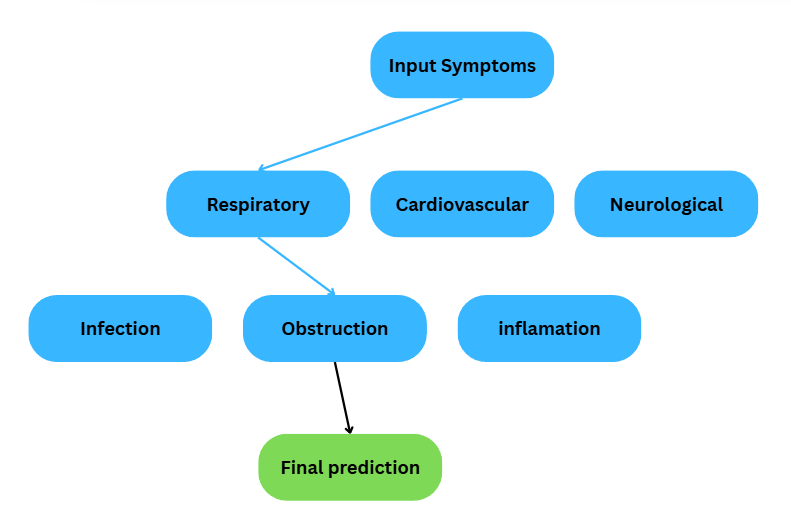
\includegraphics[width=0.7\textwidth]{Pictures/hierarchy.png}
    \caption{Flowchart for Hierarchical Classification model.}
    \label{fig:myimage}
\end{figure}

\section{Summary}

The methodology integrates structured scenario loading, multi-agent interaction, bias modelling, and LLM-mediated evaluation into a unified clinical simulation pipeline. By closely mirroring the iterative nature of real diagnostic reasoning and enabling fine-grained behavioural analysis, the system provides a robust and extensible platform for evaluating the diagnostic capabilities and limitations of open-source LLMs.